\newpage
\section{Appendix}
\subsection{Figures and graphs}
\begin{figure}[H]
    \centering
    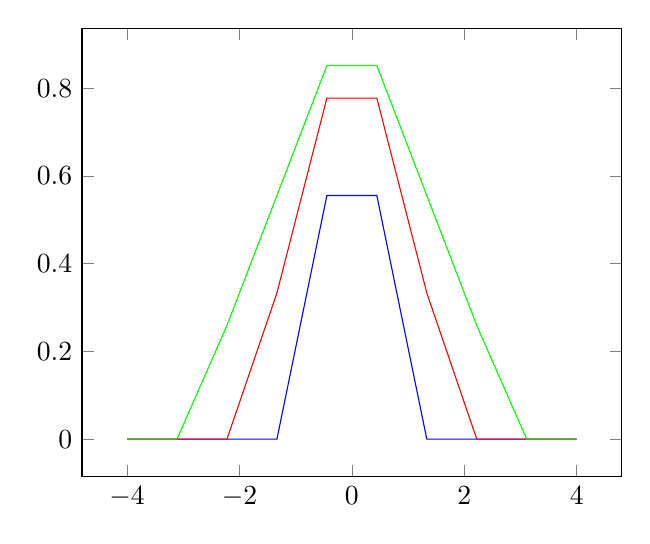
\begin{tikzpicture}
    \begin{axis}
    \addplot[domain=-4:4, samples=10, color=blue,]{max(x-1,0) + max(x+1,0) - 2*max(x,0)};
    \addplot[domain=-4:4, samples=10, color=red,]{max(x/2-1,0) + max(x/2+1,0) - 2*max(x/2,0)};
    \addplot[domain=-4:4, samples=10, color=green,]{max(x/3-1,0) + max(x/3+1,0) - 2*max(x/3,0)};
    \end{axis}
\end{tikzpicture}
    \caption{Illustration of the so-called ``bump'' function $\psi_a(x)$ used in the proof of \cref{lem:encoding-indicator-func2}. Here the colors of the displayed functions correspond to the parameter $a$ set to $a:=1$ in blue, $a:=2$ in red and $a:=3$ in green.}
    \label{fig:bump_function}
\end{figure}

\subsection{Proofs}

\begin{proof}[Proof of \cref{lem:composition_lemma}]
    Let $\cC$ be a collection of functions computed by $\wlnn$, $h_1, \dots ,h_n \in \cC$, and $\mlp^\bullet$ a multilayer perceptron. Further, let $f_{1}, \ldots, f_{n}$ be the encoding functions, as well as $\text{MLP}_1, \ldots, \text{MLP}_n$ be the multilayer perceptrons used by $h_1, \dots h_n$ respectively. As outlined above, we will now construct $f^*$ and $\mlp^*$, such that for all graphs $G \in \cX$:
    \begin{equation*}
        \mlp^\bullet(h_1(G), \dots ,h_n(G)) = \mlp^* \circ f^* \circ \wl(G)
    \end{equation*}
    such that we can conclude that the composition of multiple functions computable by $\wlnn$, is in fact also $\wlnn$ computable. 

    We define the new encoding function $f^*$ to work as follows on input $C_\infty$:
    \begin{equation*}
        f^*(C_\infty) := \textsf{concat}(
            \begin{bmatrix}
                f_1(C_\infty)\\
                \vdots\\
                f_n(C_\infty)
            \end{bmatrix}),
    \end{equation*}
    where $\textsf{conccat}$ is the concatenation functions, concatenating all encoding vectors to one single vector.

    Using the decomposition introduced in \cref{def:mlp}, we can decompose each $\mlp_i$ at layer $j > 1$ as follows: $(\mlp_i)_{j}(v) := \sigma(W^{i}_{j} \cdot (\mlp_i)_{j-1}(v) + b^i_j)$. Using this notation we construct $\mlp^*$ as follows:
    \begin{align*}
        &(\mlp^*)_{1}(v) := v\\
        &(\mlp^*)_{j+1}(v) := \sigma(W^*_j \cdot (\mlp^*)_{j} (v) + \textsf{concact}(
            \begin{bmatrix}
                b^1_j\\
                \vdots\\
                b^n_j
            \end{bmatrix})) &,\forall j \in [k]\\
        &(\mlp^*)_{j+k+1}(v) := (\mlp^\bullet)_{j+1}(v) &,\forall j \in [k^\bullet - 1]
    \end{align*}
    where $k$ is the maximum number of layers of the set of $\mlp_i$'s, $k^\bullet$ is the number of layers of the given $\mlp^\bullet$ and $\sigma$ an element wise activation function. Thereby, we define in the first equation line, that the start of the sequence is the input, with the second line, we construct the ``simultaneous'' execution of the $\mlp_i$'s, and in the last equation line, we add the layers of the given $\mlp^\bullet$ to the end. Further, we define the weight matrix $W_j^*$ as follows: 
    \begin{align*}
        W^*_j &:= \begin{bmatrix}
            W^1_j & 0 & \hdots & 0\\
            0 & W^2_j & \ddots & \vdots\\
            \vdots & \ddots & \ddots & 0\\
            0 & \hdots & 0 & W^n_j
        \end{bmatrix},
    \end{align*}
    such that we build a new matrix where each individual weight matrix is placed along the diagonal. Here we denote with $0$, zero matrices with the correct dimensions, such that $W_j^*$ is well-defined. Important to note, should for an $\mlp_i$, $W^i_j$ not exist, because it has less than $j$ layers, we use for $W^i_j$ the identity matrix $I_m$ where $m$ is the dimension of the output computed by $\mlp_i$.


    Then $\cB(\cdot) := \mlp^* \circ f^* \circ \wl(\cdot)$ is $\wlnn$ computable and equavalent to $\mlp^\bullet(h_1, \dots, h_n)$ \todo{fine tune.}
\end{proof}